
\documentclass[twoside]{ctuthesis}



\usepackage{textcomp}
\usepackage{xfrac}
\usepackage{algorithm,algorithmic}
%\usepackage[unicode]{hyperref}
\newcommand{\spc}[2]{$\mathbb{#1}^{#2}$}
\newcommand{\minsp}[3]{$\mathbb{#1} \in \mathbb{#2}^{#3}$}
\newcommand{\tl}[1]{$\mathbf{#1}$}
\newcommand{\norm}[1]{\left\lVert#1\right\rVert}


\ctusetup{
	preprint = \ctuverlog,
%	mainlanguage = english,
    titlelanguage = czech,
	mainlanguage = czech,
	otherlanguages = {slovak,english},
	title-czech = {Detekce objektů z hloubkové kamery},
	title-english = {Object Detection from Depth camera},
	%subtitle-czech = {Cesta do tajů kdovíčeho},
	subtitle-english = {Journey to the who-knows-what wondeland},
	doctype = B,
	faculty = F3,
	department-czech = {Katedra kybernetiky},
	department-english = {Department of Cybernetics},
	author = {Lukáš Kunt},
	supervisor = {Dr. Petr Štěpán},
	supervisor-address = {Ústav X, \\ Uliční 5, \\ Praha 99},
	%supervisor-specialist = {John Doe},
	fieldofstudy-english = {Mathematical Engineering},
	subfieldofstudy-english = {Mathematical Modelling},
	%fieldofstudy-czech = {Matematcké inženýrství},
	subfieldofstudy-czech = {Kybernetika a robotika},
	keywords-czech = {slovo, klíč},
	keywords-english = {word, key},
	day = 11,
	month = 5,
	year = 2020,
	%specification-file = {ctutest-zadani.pdf},
%	front-specification = true,
%	front-list-of-figures = false,
%	front-list-of-tables = false,
%	monochrome = true,
%	layout-short = true,
}

\ctuprocess

\addto\ctucaptionsczech{%
	\def\supervisorname{Vedoucí}%
	\def\subfieldofstudyname{Studijní program}%
}

\ctutemplateset{maketitle twocolumn default}{
	\begin{twocolumnfrontmatterpage}
		\ctutemplate{twocolumn.thanks}
		\ctutemplate{twocolumn.declaration}
		\ctutemplate{twocolumn.abstract.in.titlelanguage}
		\ctutemplate{twocolumn.abstract.in.secondlanguage}
		\ctutemplate{twocolumn.tableofcontents}
		\ctutemplate{twocolumn.listoffigures}
	\end{twocolumnfrontmatterpage}
}

% Theorem declarations, this is the reasonable default, anybody can do what they wish.
% If you prefer theorems in italics rather than slanted, use \theoremstyle{plainit}
%\theoremstyle{plain}
%\newtheorem{theorem}{Theorem}[chapter]
%\newtheorem{corollary}[theorem]{Corollary}
%\newtheorem{lemma}[theorem]{Lemma}
%\newtheorem{proposition}[theorem]{Proposition}

%\theoremstyle{definition}
%\newtheorem{definition}[theorem]{Definition}
%\newtheorem{example}[theorem]{Example}
%\newtheorem{conjecture}[theorem]{Conjecture}

%\theoremstyle{note}
%\newtheorem*{remark*}{Remark}
%\newtheorem{remark}[theorem]{Remark}

%\setlength{\parskip}{5ex plus 0.2ex minus 0.2ex}

\begin{document}
\maketitle

%\part{Teoretická část}
%\chapter{Teoretická část}
\chapter{Matematický aparát}
\section{Homogenní souřadnice}
Během celé práce budu pracovat jak s kartéskými, tak i s homogenními souřadnicemi. Tyto jsou v Euklidovském prostoru dimenze $n$ reprezentovány pomocí vektoru, který má $n+1$ prvků. Je-li $\boldsymbol{r}$ bod v trojdimenzionálním Euklidovském prostoru $\mathbb{E}^3$ reprezentován parametry $x,y,z$, pak pro převod mezi kartézskými a homogenními souřadnice platí následující vztahy.
\begin{align}
    \mathbf{r} = \begin{bmatrix} x \\ y \\ z \end{bmatrix} &\rightarrow \mathbf{r}_{hom} = \begin{bmatrix} x \\ y \\ z \\ 1 \end{bmatrix} \\
    \mathbf{r}_{hom} = \begin{bmatrix} x \\ y \\ z \\ w \end{bmatrix} &\rightarrow \mathbf{r} = \begin{bmatrix} \sfrac{x}{w} \\ \sfrac{y}{w} \\ \sfrac{z}{w} \end{bmatrix}
\end{align}
Pomocích homogenních souřadnic můžeme sestavit transformační matici \tl{A} , takto se skládá z matice rotace \tl{R} a vektoru translace \tl{t}.
\begin{align}
    \mathbf{A} = \begin{bmatrix} \mathbf{R} & \mathbf{t} \\ \mathbf{0} & 1 \end{bmatrix}
\end{align}

\section{Rotace a rotační matice}
Natočení souřadného systému, popřípadě objektu s tímto svázaným vhledem k jinému systému v prostoru dimenze $n$ se nejjednodušeji popíše pomocí rotační matice \tl{R} $\in$ \spc{R}{n}. Mezi nejběžnější rotační matice patří rotace o úhel $\theta$ kolem os kartézského souřadného systému v \spc{E}{3}. Tyto vypadají následovně.
\begin{align}
    \mathbf{R_x}=\begin{bmatrix} \cos \theta & -\sin \theta & 0 \\ \sin \theta & \cos \theta & 0 \\ 0 & 0 & 1 \end{bmatrix} \\
    \mathbf{R_y}=\begin{bmatrix} \cos \theta & -\sin \theta & 0 \\ \sin \theta & \cos \theta & 0 \\ 0 & 0 & 1 \end{bmatrix} \\
    \mathbf{R_z}=\begin{bmatrix} \cos \theta & -\sin \theta & 0 \\ \sin \theta & \cos \theta & 0 \\ 0 & 0 & 1 \end{bmatrix}
\end{align}
Obecné natočení pak můžeme dostat složením 3 a více těchto rotací \footnote{Na pořadí zde záleží, není možné dostat libovolnou rotační matici, pokud budou dvě po sobě doucí rotace probíhat kolem stejné osy}
Pro vytvoření matice rotace \tl{R} v prostoru \spc{R}{3} kolem obecné osy dané normalizovaným vektorem \tl{u} o úhel $\theta$ slouží Rodriguesův vzorec \cite{RodriguesRotationFormula}.
\begin{align}
    \mathbf{R} = \mathbf{I} + \tilde{\mathbf{u}}\sin \theta + \tilde{\mathbf{u}}^2(1 - \cos \theta); \quad \tilde{\mathbf{u}} = \begin{bmatrix} 0 & -u_{z} & u_{y} \\ u_z & 0 & -u_x \\ -u_y & u_x & 0 \end{bmatrix}
    \label{Rodriguez}
\end{align}
Chceme-li natočit vektor \tl{a} tak, aby byl rovnoběžný s vektorem \tl{b} použijeme vzorec \ref{Rodriguez}, úhel rotace $\theta$ a vektor \tl{v} kolem kterého rotace proběhne se určí následovně.
\begin{align}
    \mathbf{v} = \frac{\mathbf{a} \times \mathbf{b}}{\norm{\mathbf{a}\times \mathbf{b}}}\\
    \theta = \arccos \left( \frac{\mathbf{a} \cdot \mathbf{b}}{\norm{\mathbf{a}}\norm{\mathbf{b}}} \right)
\end{align}
Podle \cite{james_w_angle_2014} je tato metoda nevhodná pro výpočet na počítači. Zejména pak v případech, kdy bychom měli počícat $\arccos$ hodnot blízko $\pm 1$. Toto je způsobeno omezonou přesností reprazentace desetinných čísel v počítači (takzvaná floating point aritmetika). Přesnější je tedy použít tento vzorec.
\begin{align}
    \theta = \text{atan2}\left( \norm{\mathbf{a} \times \mathbf{b}}, \mathbf{a}\cdot \mathbf{b} \right) 
\end{align}
Výhoda funkce atan2 oproti arcus tangens je oštřené dělení nulou, ke ktrému může dojít při zaokrouhlování desetiných čísel. Navíc funkce vrací úhel v rozmezí $\left[ 0, 2\pi \right]$

\section{Vlastní čísla a vektory}
Pro čtvercovou matici \minsp{A}{R}{n\times n} a nenulový vektor \tl{v}\minsp{}{R}{n} a sklár $\lambda \in \mathbb{R}$ platí
\begin{align}
    \mathbf{Av} = \lambda \mathbf{v}.
\end{align}
Skalár $\lambda$ se nazývá vlastní číslo matice \tl{A} a vektor \tl{v} vlastní vektor příslušný vlastnímu číslu $\lambda$.
Spektrální věta (viz. \cite{Werner2020}) říka: Je-li matice \tl{A} symetrická, pak má $n$ vlastních čísel, kde $n = \text{rank}\mathbf{A}$ a všechna vlastní čísla jsou reálná.

\section{Singulární rozklad}
Singulární SVD\footnote{Z anglického Singular Value Decomposition}rozklad umožní každou matici \tl{A} $\in$ \spc{R}{m \times n} rozložit jako
\begin{align}
    \mathbf{A} = \mathbf{USV}^T
\end{align}
kde matice \tl{S} je diagonální, matice \tl{U} je ortogonální a obsahje vlastní vektory matice \tl{AA}$^T$, obdobně je pak i matice \tl{V} ortogonální a je složena z vlastních vektorů matice \tl{A}$^T$\tl{A}

\section{Analýza hlavních komponent}
Analýza hlavních komponent (PCA\footnote{Z anglického Principal Component Analysis}) 

\chapter{Kamera}

\section{Dírkový model kamery}
Kamera zobrazuje body \tl{p} $\in \mathbb{E}^3$ na $\mathbf{p}_{o} \in \mathbb{E}^2$. Je to tedy zobrazení mapující body ve světovém souřadném systému na body v souřadném systému obrazu kamery. Nejjednodušším modelem je dírkový. Jedná se o model kamery s konečný optickým centrem, neboli centrem projekce. Toto umístíme do počátku kartézského souřadného systému a budeme uvažovat plochu kolmou na osu $Z$ našeho souřadného systému, kterou nazveme obrazovou rovinou tato je popsána jediným parametrem a to ohniskovou vzdáleností $f$. V dírkovém modelu kamery se bod v prostoru \tl{p} = $(x,y,z)^T$ zobrazí na bod obrazu pomocí následující zobrazení
\begin{align}
    \begin{bmatrix} x \\ y \\ z \end{bmatrix} \mapsto \begin{bmatrix} \sfrac{fx}{z} \\ \sfrac{fx}{z} \end{bmatrix}
    \label{pinhole_eq}
\end{align}
což odpovídá bodu, kde přímka spojující centrum projekce a bod v prostoru, protne obrazovou rovinu (viz obrázek \ref{pinhole}). Ve vztahu \ref{pinhole_eq} jsme předpokládali, že počátek souřadného systému obrazu je v optickém středu. Většinou se však za počátek souřadnic volí levý horní roh obrazu. K zápisu využijeme homogenních souřadnic a dostaneme následující rovnici
\begin{align}
    \begin{bmatrix} x \\ y \\ z \\ 1 \end{bmatrix} \mapsto \begin{bmatrix} fx + zc_x \\ fy + zc_y \\ z \end{bmatrix} = \begin{bmatrix} f & 0 & c_x & 0 \\ 0 & f & c_y & 0 \\ 0 & 0 & 1 &0 \end{bmatrix} \begin{bmatrix} x \\ y \\ z \\ 1 \end{bmatrix}
    \label{pinhole_homogenous}
\end{align}
kde jako $c_x$ a $c_y$ jsme označili souřadnice optického středu. Označíme-li obecný bod v prostoru,který je popsán v souřadném systému kamer \tl{x}$_p$ a odpovídající bod v rovině obrazu \tl{x}, pak můžeme rovnici \ref{pinhole_homogenous} přepsat jako
\begin{align}
    \mathbf{x} = \mathbf{K}[\mathbf{I}\; |\; 0 ]\mathbf{x}_p \quad \mathbf{K} = \begin{bmatrix} f & 0 & c_x  \\ 0 & f & c_y  \\ 0 & 0 & 1  \end{bmatrix}
    \label{intrinstic}
\end{align}
Matice \tl{K} se nazýva matice vnitřních parametrů kamery.

Obecně je bod v prostoru $\mathbf{x}$ popsán v jiném souřadném systému, než je ten se kterým je svázána kamera, tento se nejčastěji nazývá světový souřadný systém. Přechod do souřadného systému kamery ze světového je možno popsat následovně 
\begin{align} 
    \mathbf{x}_p = \begin{bmatrix} \mathbf{R} & -\mathbf{R\tilde C} \\ 0 & 1 \end{bmatrix}
    \mathbf{x}
    \label{world_to_cam}
\end{align}
Kde jsme jako $\tilde{\mathbf{C}}$ označili počátek souřadného systému kamery vyjádřený v světových souřadnicích a \tl{R} rotaci světového souřadného systému vzhledem k kameře. Dosadíme-li nyní rovnici \ref{intrinstic} do \ref{world_to_cam} dostane vztah popisující transformaci bodu z světových souřadnic do souřadnic obrazu.
\begin{align}
    \mathbf{x} = \mathbf{KR}[\mathbf{I} \; | \; - \mathbf{\tilde C} ]\mathbf{x}
    \label{world_to_img}
\end{align}
Parametry $\mathbf{\tilde C}$ a \tl{R} se souhrně nazývají vnější parametry kamery. 
\begin{figure}
    \centering
    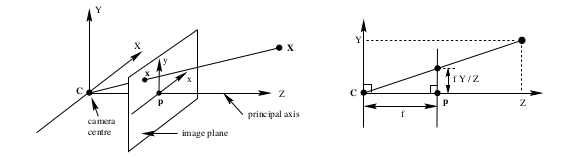
\includegraphics[width = 0.8\linewidth]{pictures/dirkovymodel_nakres.png}
    \caption{Model dírkové kamery}
    \label{pinhole}
\end{figure}

\section{Stereo kamera}
\subsection{Výpočet vzdálenosti}
Stereo kamera je tvořena dvěma nezávislými čočkami. Zpracováním obrazů jsme schopní získat informaci o hloubce každého bodu obrazu. Budeme uvažovat model stereo kamery, kde osy obou čoček jsem rovnoběžné (viz obrázek \ref{stereo_paralel}). Osy jsou od sebe ve vzdálenosti $b$, tomuto parametru se říka základní linie (baseline).Z podobnosti trojúhelníků plyne
\begin{align}
    \frac{z}{f} = \frac{x}{xl} \label{trojuh1} \\
    \frac{z}{f} = \frac{x - b}{xr} \label{trojuh2}
\end{align}
pokud z rovnice \ref{trojuh1} vyjádříme $x$ a dosadíme do rovnice \ref{trojuh2}, pak po úpravě dostaneme výsledný vztah pro vzdálenost bodu od kamery. Hodnota d se pak nazývá rozdíl (disparity).
\begin{align}
    z = \frac{fb}{xl - xr} = \frac{fb}{d} 
    \label{depth_stero}
\end{align}
Kde $xl$ a $xr$ jsou souřadnice bodu \tl{p} v levém a pravém obrazu stereokamery. Pro každý bod v levém (popřípadě pravém) obrazu je tedy potřeba najít odpovídající bod v obrazu pravém (tzv. stereo pár). Bez jakékoliv apriorní znalosti by to znamenalo pro každý pixel prohledat celý druhý obraz, tedy náročnost hledání $\mathcal{O}(wh)$.Pomocí epipolární geometrie můžeme hledání zúžit na přímku  a snížit tak náročnost hledání stero páru na $\mathcal{O}(w)$.

\subsection{Chyba výpočtu vzdálenosti}
Chyba výpočtu vzdálenosti se podle \cite{keselman2017intel} určí derivací rovnice \ref{depth_stero} podle $d$.
\begin{align}
    \frac{\partial z}{\partial d} = \frac{z}{fb} \\
    |\epsilon_z | = \frac{z^2}{fb}|\epsilon_d |
    \label{error_stereo}
\end{align}
Kde $\epsilon_z $ je chyba určení vzdálenosti bodu a $ \epsilon_d $ je chyba rozdílu, toto je vlastnost kamery, popřípadě algoritmu požitého ke hledání odpovídající párů (viz. TODO fill secetion) a nabývá téměř konstantních hodnot \cite{keselman2017intel}. Z \ref{error_stereo} tedy plyne, že chyba je úměrná kvadrátu vzdálenosti daného bodu a přesnost stereo kamer se vzdáleností rychle klesá.

\subsection{Epipolární geometrie}
\label{Sec:epipolar}
Epipolární geometrie se zabývá průnikem obrazových rovin a svazkem ploch, jejichž společná osa je báze. Uvažujme dvě dírkové kamery v obecném natočení, tedy jejich obrazové roviny nemusí být rovnoběžné (viz \ref{fig:epipolar}). Z dírkové modelu kamery plyne, že bod \tl{X} a optické středy kamer $C, C'$ jsou koplanární a tvoří rovinu $p$. V místě, kde tato rovina protíná rovinu obrazu se nachází epipolární přímka $l$. Hledáme-li stereo pár, pak pro známý bod \tl{x} (tj. projekce bodu \tl{X} do optické roviny levé kamery) musíme najít odpovídající bod \tl{x'}. Tento může ležet pouze na epipolární přímce $l'$. Přímka $l'$ je uřčna epipólem $e'$ a bodem $x'$. Epipól se nachází v místě, kde přímka spojující optickcká centra kamer protíná rrovinu obrazu. Bod $x'$ se určí jako 
\begin{align}
    \mathbf{x'} = \mathbf{Hx}
\end{align}
Kde \tl{H} je homografie mezi rovinami obrazu . Toto mapování je ovlivněno pouze vzájemnou polohou kamer a jejich vnitřními parametry a nezávisí tedy na scéně.
Z bodu \tl{x'} se pak již určí epipolární přímka \tl{l'}.
\begin{align}
    \mathbf{l'} = \mathbf{e'} \times \mathbf{x'} \\
    \mathbf{l'} = \mathbf{e'} \times \mathbf{Hx} \\
    \mathbf{l'} = \mathbf{Fx} 
\end{align}    
Matice \tl{F} se nazývá fundamentální a $\text{rank}\,{\mathbf{F}} = 2$, tedy zobrazení reprezentované maticí F zobrazí bod na přímku.
    Pokud jsou obě optické osy stereo kamery rovnoběžné, pak se výpočet epipolární přímky velice zjednodušší, jelikož homografie mezi rovinami obrazu je pouze posunem ve směru báze.
\begin{figure}

    \centering
    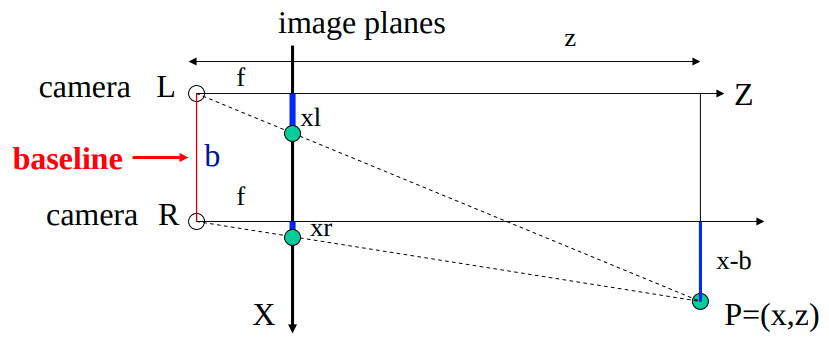
\includegraphics[width = 0.8\linewidth]{pictures/stereo_sketch.png}
    \caption{\cite{washingtion_steropic}}
    \label{stereo_paralel}
\end{figure}
\section{Hledání stereo páru}
Metody užívané pro hledání stereo parů se dělí na metody plošné (area based) a ty založené na porovnávání rysů (features). Při hledání stereo páru se často využívá následujících omezení, která tento proces zjednodušší. Tato však v extrémních případech nemusí platit.
\begin{itemize}
    \item Epipolární omezení: pixel v druhém obrazu se nachází ( pokud existuje ) na epipolární přímce (vit. \ref{Sec:epipolar})
    \item Spojitost: Rozdílová, popř. hloubková mapa by měla být po částech spojitá.
    \item Jedinečnost: Každý pixel v levém obrazu má k sobě právě jeden odpovídající v obrazu pravém. 
    \item Pořadí: Pořadí pixelů v levém obraze odpovídá pořadí v ptavém
\end{itemize}

\subsection{Plošné metody}
Využívají informaci z okolí pixelu. Tyto jsou porovnány se všemi možnými pozicemi v druhém obrazu a bod, jehož hodnota je nejblíže vzoru rvoří stereo pár. Mezi nejpoužívanější algoritmy patří.

\subsubsection{Součet absolutních rozdílů}
Je definována konstatní velikost okolí pixelu $\mathbf{x}(u,v)$, pro který se hledá stereo pár. Tato je následně porovnávána s body, kde se může korespondující pixel nacházet, tj. body které splnují námi požívaná omezení. Pro odpovídající bod \tl{x'} tedy platí následující vztah. 
\begin{align}
    \mathbf{x'} = \text{argmin}\left( \displaystyle\sum_i \displaystyle\sum_j |\mathbf{I}_l(u+i,v+j) - \mathbf{I}_r(u+i, v+j + d)| \right)
\end{align}
kde $\mathbf{I}(u,v)$ je intenzita příslušného pixelu, $d$ je posun okna ve druhém obrazu a součet probíha přes celé okno, tedy přes každé $i,j$. Vztah byl zjednodušen uvažováním horizontálních epipolárních přímek. To odpovídá konfiguraci kamery s rovnoběžnými optickými osami.

Existuje spoustu podobných algoritmů, které pouze používají jinou metrickou funkci. Místo absolutní hodnoty například kvadrát rozdílu, nebo normalizovaný kvadrát rozdílu. Všechny tyto metody patří mezi nejpřesnější \cite{kuhl2005comparison}. 

\subsubsection{Cenzus}
\label{Sec:cenzus}
Tato metoda opět pracuje se definovanou maskou kolem pixelu, pro který hledá stero pár. Pixely, které se nachází v šabloně se přemění na vektor jedniček a nul, podle toho zda je hodnota intenzita větší, popřípadě menší než intenzita centrálního pixelu. Stejná transformace se provede i v pravém obrazu pro každý pixel, který může doplnit stereo pár. Vektory jsou následně porovnány a je vybrán ten, jehož vektor má nejmenší Hammingovu vzdálenost.

\subsection{Porovnávání rysů}
Pro každý obraz jsou vygenerovány důležité body. Tyto mohou být nepříklad hrany či rohy. Tyto jsou porovnány s analogicky vygenerovánými rysy v druhém obrazu. Využívá se algoritmů jako je například SIFT (Scale Invariant Feature Transform), SURF (Seeded-Up Robust Features) nebo BRIEF(Binary Robust Independent Elementary Features)

\begin{figure}
    \centering
    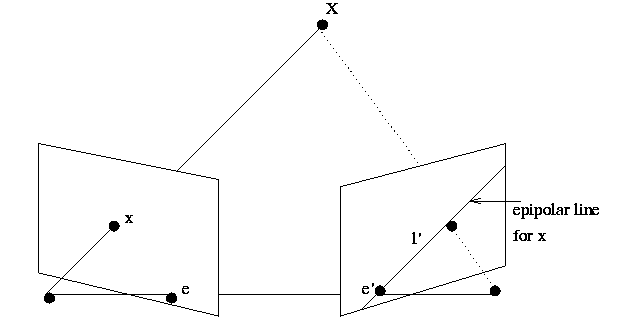
\includegraphics[width = 0.8\linewidth]{pictures/epipolar.png}
    \caption{Placeholder}
    \label{fig:epipolar}
\end{figure}
%TODO uncoment this ( avoiding compilation warnings )




%\section{Intel \textregistered Realsense\textsuperscript{TM} D435}
\section{Intel Realsense D435}
Intel\textregistered{} Realsense\textsuperscript{TM} D435 je širokoúhlá stereo kamera, která se skládá z RGB kamery, infračerveného (infra red )projektoru, a dvou infračervených kamer jejichž data zpracovává přímo v čipu kamery procesor. Výstupem z kamery je tedy barevný obraz (RGB) a vzdálenost jednotlivých pixelů (hloubková mapa). 

\begin{figure}
    \centering
    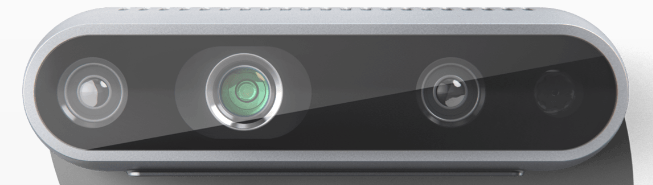
\includegraphics[width = 0.8\linewidth]{pictures/realsense_kamera.png}
    \caption{Fotografie kamery Intel\textregistered{} Realsense\textsuperscript{TM} D435 \cite{Realsense_obrazek}}
    \label{Fig:realsense_pic}
\end{figure}

    Dvě infračervené kamery jsou v konfiguraci s rovnoběžnými optickými osami ve vzdálenosti 50$\,mm$. Infračervený projektor promítá na scénu statický obrazec, který se nachází mimo viditelné spektrum a není tedy zachycen RGB kamerou. Tento obrazec slouží k najítí stereo párů, zejména pak u objektů s řídkou texturou.

    Kamera je vybavena specializovaným procsorem Vision Processor D4 pro výpočet hloubkové mapy. Tento je schopen při rozlišení hloubkové kamery 848x480 zpracovávat až 90 snímků za sekundu (FPS) \cite{RealSense_datasheet}, toto je vykoupeno sníženou přesností \cite{keselman2017intel} a pro maximální přesnost je vhodné snížit frekvenci na 30 snímků za sekundu.  Procesor má stejně jako celá kamera velice nízký odběr. Celá kamera včetně IR projektor má odběr menší než jeden watt a je tedy vhodná pro mobilní aplikace, kde je velikost baterie a spotřeba energie omezujícím faktorem.

    Pro hledání stereo párů je využit cenzus algoritmus popsaný v \ref{Sec:cenzus} s maskou velikosti $7 \times 7 $. Výsledky jsou následně ověřovány sadou filtrů, které měří důvěryhodnost shody. Podle nastaveného limitu pak pro tento pixel bud vygenerují záznam v hloubkové mapě, nebo pixel zůstane nevyplněn. Výsledky kamery pro různé hodnoty limitu jsou vidět v tabulce. 
\begin{figure}
    \centering
    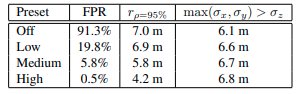
\includegraphics[width = 0.8\linewidth]{pictures/realsense_threshold.png}
    \caption{Postupně zleva: hodnota limitu, počet falešných shod pokud je scéna blíže, než je minimální vzdálenost detekce kamerou. Vzdálenost, kdy vyplněnost hloubkové mapy klesne pod $95\%$ a vzdálenost při které je směrodatná odchylka ve směru osy $z$ menší, než ve směru $x$ a $y$ \cite{keselman2017intel}}
    \label{fig:tablka_limity}
\end{figure}

Procesor kamery není schopen určit hloubku bodu, pokud se objekt nachází příliš blízko. Konkrétní hodnoty je možno vidět v tabulce \ref{Fig:minimalni_hloubka}. Maximální měřitelná vzdálenost je za ideálních podmínek až 40 metrů \cite{keselman2017intel}. S rostoucí vzdáleností se kamera chová podle rovnice \ref{error_stereo}, toto chvání není patrné, pokud kamera operuje s objekty, které se nachází na obou hranicích měřitelné vzdálenosti, viz

\begin{figure}
    \centering
    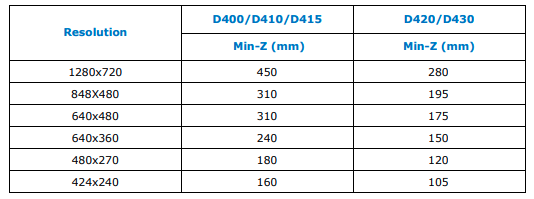
\includegraphics[width = 0.8\linewidth]{pictures/minimalni_vzdalenost.png}
    \caption{Tabulka minimální detekovatelné hloubky \cite{RealSense_datasheet}}
    \label{Fig:minimalni_hloubka}
\end{figure}

\section{Matody v detekci objektů}
\subsection{Určování normálového vektoru}
Ve většině scén počitačového vidění lze pozrovat velké plochy, jakými jsou například stěny, či zem. Tyto jsou důležitým blokem pro většinu postupů detekce objektů. Například přesné určení směru podložky je nezbytné pro detekci objektů ležících na této podložce. Rozlišujeme dva časté postupy: Již známe body, které jsou součástí dané plochy, tj. již byla provedena segmentace obrazu, nebo 

\section{Výpoet normálového vektoru plochy nerganizovného mračna bodů} 
Normálový vektor plochy je definován, jako vektor kolmý na každý vektor dané plochy. 
\section{RANSAC}
    Výpočet normálového vektoru v bodě proběhne selekcí $n$ bodů jejichž vzdálenost od 

\section{Zvolený postup}
Bylo navrženo a implementováno několik postupů. Tyto se dělí do dvou kategorií.
\begin{itemize}
    \item Segmentace obrazu na skupiny bodů odpovídající jednotlivým cihlám
    \item Detekce samotné cihly a její vizualizace pomocí ohraničujícího boxu
\end{itemize}

\subsection{Segmentace obrazu}
\subsubsection{Přístup založený na výšce}
Tento postup vychází z předpokladu, že na zami se krom cihel nanachází jiné předměty. Scénu tedy tvorí pouze zem a na ní umístěné cihly, které mají předem známé rozměry. Začneme určením normálového vektoru roviny reprezentující zem, jelikož z jeho znalosti můžeme najít body ležící nad zemí, tj. body představující cihly. 
Vytvoříme mřížku bodů, které jsou v místech, kde předpokládáme přesný výstup kamery. U těchto ověříme, zda pro ně byla kameoru vygenerována hloubka, dále ověřme, zda bod leží v maximální vzdálenosti 4\,, jelikož podle \cite{} a (ref to realsense) chyba stereo kamery nad tuto vdálenost začíná být markantní a správné určení normálového vektoru je zásadní pro všechny ostatní kroky. Množinu bodů $M = \mathbf{a}_1 \dotsc \mathbf{a}_m$ které splňují výše uvedná kritéria proložíme rovinou pomocí PCA algoritmu a dostaneme tedy normálový vektor \tl{n} plochy $p$ minimalizující kvadrát vzdáleností od bodů tato je posunuta mimo počátek o $d$.
\begin{align}
    \mathbf{\bar{a}} = \frac{1}{m}\left( \mathbf{a}_1 \dotsc \mathbf{a}_m \right) \\
    d = \mathbf{n} \cdot \mathbf{\bar{a}} = \mathbf{n}^T \mathbf{\bar{a}} \\
    p: n_1x + n_2y + n_3z - d = 0 \label{normal_plane}
\end{align}
Každý bod \tl{a} je buď součástí země, nebo součastí cihly. Je-li v množině $M$ $k$ bodů, které jsou součastí země $G$, pak zbylých $m - k$ bodů musí být součastí mračna bodů reprezentující cihlu $C$. Tyto body se vždy nachází ve výšce $z$ \footnote{Osa z směřuje směrem z kamery a tedy body nacházající se nad zemí mají menší hodnotu $z$}nad zemí a tedy platí, pro každý bod \tl{a}
\begin{align}
    n_1a_1 + n_2a_2 + n_3a_3 + \epsilon > d \; \rightarrow \; \mathbf{a} \in C  \\
    n_1a_1 + n_2a_2 + n_3a_3 + \epsilon \leq d \; \rightarrow \; \mathbf{a} \in G  
\end{align}
Kde $\epsilon$ je experimentálně určená hodnota, která oštří případy, kde $k = m$, tj. všechny body reprezentují zem. V tomto případě čast bodů bude ležet na plochou $p$. To jest dáno šumem dat a nepřesností kamery. Přidáním parametru $\epsilon$ je zajištěno, že každý bod reprezentující zem bude registrován.

Po výběru bodů z mřížky podle výše uvedených kriterií dostaneme $k$ bodů, které reprezentují zem a nacházejí se v místech, kde je přesnost kamery v rámci jejich možností nejvyšší. Tyto body by se daly znovu proložit plochou a dostat tak aproximaci natočení země pomocí normálového vektoru \tl{n}. Vzhledem k důležitosti přesnosti určení \tl{n} získáme další body reprezentující zem pomocí algoritmu \ref{alg:floodfill}. Tyto pody opět pomocí PCA proložíme přímkou a dostaneme dobrou aproximaci normálového vektoru země. Na obrázku je vidět výsledek algoritmu \ref{alg:floodfill}.
    
    
\begin{algorithm}
    \caption{Epadndování bodů}
    \label{alg:floodfill}
    \begin{algorithmic}
        %\STATE S = stack
        %\STATE G = points that belongs to ground
        %\STATE V = visited points
        \STATE $Stack \gets \emptyset$
        \STATE $G \gets \emptyset$
        %\STATE $V \gets \emptyset$ \quad //visited points
        \FOR{$\mathbf{a}$ in $M$}
            \STATE Stack.push($\mathbf(a)$)
            \STATE $z \gets$ height of $\mathbf{a}$
            \WHILE{\NOT Stack.empt()}
                \STATE $\mathbf{t} \gets$ Stack.pop()
                \STATE $G \gets G \cup t$
                \STATE $V \gets V \cup p$
                \FOR{$\mathbf{n}$ in neighbours of $\mathbf{t}$}
                    \STATE $zn \gets$ height of $\mathbf{n}$
                    %\IF{$zn \in \left[ z - \delta , z + \delta\right]$ \AND \NOT $\mathbf{n}$ $\in V$}
                    \IF{$zn \in \left[ z - \delta , z + \delta\right]$ \AND \NOT $\mathbf{n}$ $\in G$}
                    \STATE stack.push($\mathbf{n}$)
                    \ENDIF
                \ENDFOR
            \ENDWHILE
        \ENDFOR
    \end{algorithmic}
\end{algorithm}

\begin{figure}
    \centering
    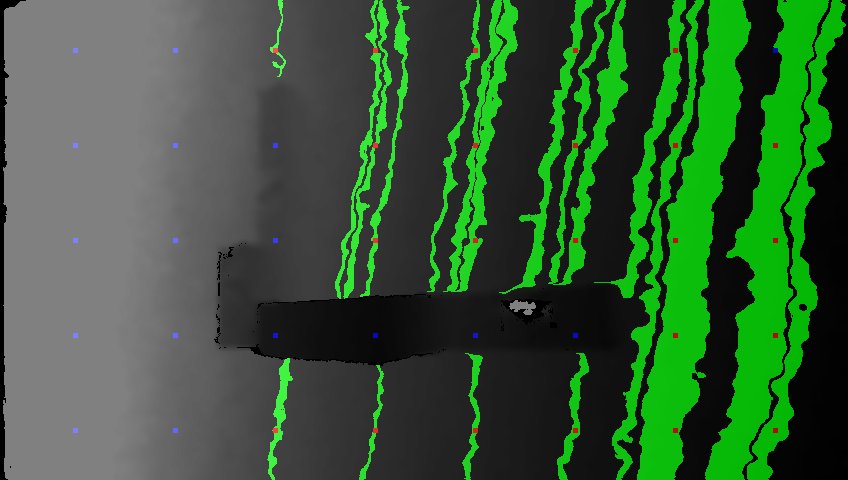
\includegraphics[width = \linewidth]{pictures/prob0001body_gnd.png}
    \caption{Červenou barvou jsou znázorněny body, ze kterých probýhal algoritmus \ref{alg:floodfill}, modré body byly podle výše uvedených kritérií vyřazeny a zeleně jsou znázorněny výsledné body reprezentující zem}
    \label{fig:floodfill}
\end{figure}

Nyní se vypočítá výška každého bodu nad rovinou a podle této hodnoty se přidělí hodnota 0 až 3, kde číslo reprezentuje očekávaný počet na sobě naskládaných cihel. Vizualizace tohoto výsledku je vidět na obrázku \ref{fig:height_map}

\begin{figure}
    \centering
    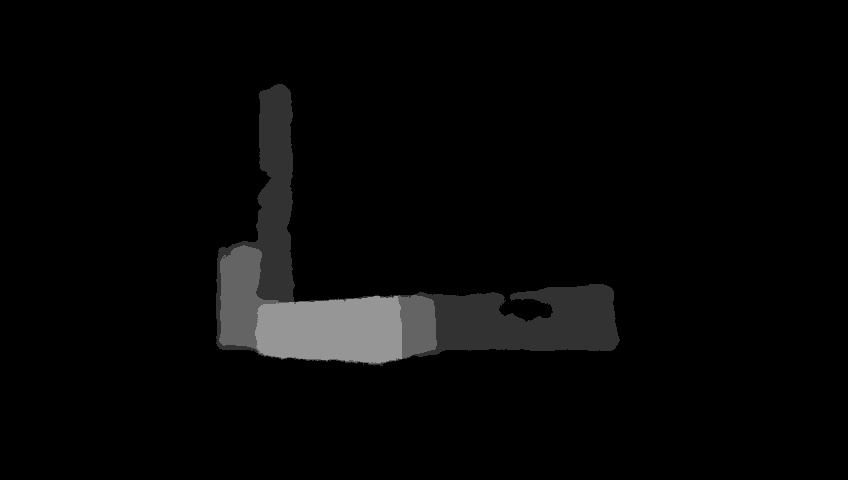
\includegraphics[width = \linewidth]{pictures/original_vrstva2_pic1.jpg}
    \caption{Vzdálenost boudů od roviny zobrazena jako počet na sobě lžících cihel}
    \label{fig:height_map}
\end{figure}

\subsubsection{Přístup založený na derivaci}



\bibliography{citations}
\bibliographystyle{plain}
\end{document}
